        Logo abaixo são apresentados os resultados da primeira iteração de avaliação do protótipo.
      
      \begin{itemize}
       \item \textbf{Descrição e metodologia do roteiro da avaliação}
       
       \subitem O objetivo dessa avaliação é analisar qual a satisfação obtida pelo usuário ao utilizar o protótipo considerando as seguintes 
       metas e princípios de usabilidade, além das heurísticas definidas por Nielsen:
       \begin{itemize}

	\item Utilidade
        \item Eficácia
        \item Eficiência
        \item Visibilidade
        \item Feedback
        
       \end{itemize}
       
       \item \textbf{Comportamento dos usuários}
       
       \subitem Ao todo, os cinco usuários que avaliaram o protótipo conseguiram cumprir todas as tarefas estabelecidas 
       de todos os cenários. Agiram perante as atividades do protótipo de maneira intuitiva, apesar de ficarem 
       desatentos em relação a alguns ícones, e não demoraram a cumprir as funcionalidades dos cenários de avaliação 
       estabelecidos.
       
       \item \textbf{Resumo das entrevistas}
       
       \subitem Alguns usuários estavam com vergonha de realizar a avaliação pelo fato de ter que fazer uma gravação em vídeo. 
       Devido a isso, foi questionado a eles se os mesmos estavam realmente seguros de realizar a avaliação ou se desejavam 
       interromper a mesma e não realizá-la. Nessa primeira iteração, nenhum dos usuários se negaram e decidiram por 
       continuar a avaliação. As avaliações foram realizadas de maneira mais rápida do que as avaliações do protótipo de papel, 
       devido ao fato de o protótipo de alta fidelidade possuir funções que o tempo de resposta se reduz e não possui mais a 
       necessidade de ficar passando folha a folha do protótipo como ocorria nas avaliações do protótipo de papel.
       
       \item \textbf{Problemas de usabilidade identificados}
       
       \subitem No momento da avaliação, através de observações feitas pela equipe e por análise nos vídeos coletados, foram percebidos 
       alguns problemas de usabilidade que os usuários estiveram no momento da interação com o protótipo. Tais como:
       
       \begin{itemize}
       
       \item Dificuldade em entender o significado do horário da notificação.
       
       \item Dificuldade em identificar o ícone para adicionar o tema da notificação.
       
       \item Dificuldade em identificar o ícone para editar uma notificação.
       
       \item Dificuldade em identificar o ícone para excluir uma notificação.
       
       \end{itemize}
       
       \item \textbf{Paradas críticas}
       
       \subitem No momento da avaliação não houve nenhum caso a qual o usuário ficou sem reação em relação à execução de algum cenário. 
       Quando os mesmos obtiveram dificuldades com alguns ícones, estes ícones foram encontrados no momento da execução.
       
       \item \textbf{Plano de correção}
       
       \subitem Para corrigir os problemas de usabilidade que foram identificados para esta iteração, a equipe vai melhoras a interface do 
       protótipo aumentando os botões dos ícones para deixá-los mais visíveis, pois assim ficará mais intuitivo para o usuário qual 
       atividade aquele ícone vai realizar.
       
      \end{itemize}
      
      Na figura \ref{asqalta} se encontram as respostas ao questionário ASQ pelos cinco usuários avaliados.
      
  \begin{figure}[!htb]
  \centering
  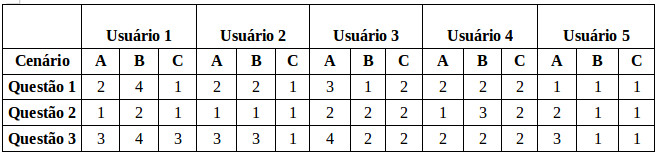
\includegraphics[scale=0.6]{figuras/asqalta.jpg}
  \caption{Resposta dos usuários ao questionário ASQ na primeira avaliação do protótipo de alta fidelidade}
  \label{asqalta}
  \end{figure}
      
      Na figura \ref{pssuqalta} se encontram as respostas ao questionário PSSUQ pelos cinco usuários avaliados.
      
  \begin{figure}[!htb]
  \centering
  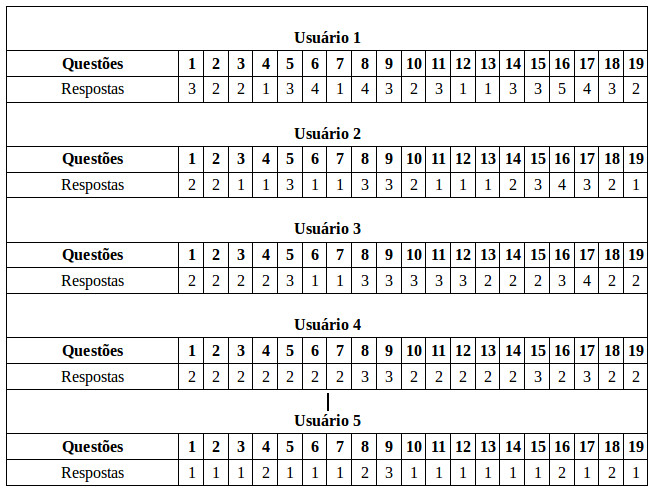
\includegraphics[scale=0.6]{figuras/pssuqalta.jpg}
  \caption{Resposta dos usuários ao questionário PSSUQ na primeira avaliação do protótipo de alta fidelidade}
  \label{pssuqalta}
  \end{figure}